\section{Wiederholung}
\label{sec:recap}

\subsection{Aufgabe 1}
\begin{frame}[fragile]
    \frametitle{\insertsubsection}
    Schreibe ein Python-Script, um die folgenden \acp{ode} numerisch zu lösen:
    \begin{equation}
        \dot{A} = k_1 - k_2 A
    \end{equation}
    \begin{equation}
        \dot{A} = k_1 - k_2 A + k_3 A^2 - k_4 A^4
    \end{equation}
    \begin{align}
        \dot{A} &= k_1 B - k_2 A\\
        \dot{B} &= k_2 A - k_1 A
    \end{align}
    Verwende dabei scipy zum lösen und matplotlib zum visualisieren
    \begin{minted}[linenos, fontsize=\scriptsize, escapeinside=||]{python}
|\pause|from scipy.integrate import odeint
import matplotlib.pyplot as plt
    \end{minted}
    Welche Werte müssen wir für eine numerische Lösung vordefinieren?
\end{frame}


\section{Reaktionsnetzwerke}
\label{sec:reaction-networks}


\subsection{Diagramm $\rightarrow$ \acs{ode}}
\label{subsec:diag_to_eq}
\begin{frame}
    \frametitle{\insertsubsection}
    \begin{itemize}[<+->]
        \item Gegeben ist eine Reaktionsnetzwerk
        \[A + A \rightarrow B\]
        \[B + C \rightarrow \varnothing\]
        \item Wie kann man diese Reaktion als \ac{ode} ausdrücken?
        \item Was ist die Lösung der \ac{ode}?
        \item Was sind die charakteristiken der \ac{ode}?
    \end{itemize}
\end{frame}


\subsection{Beispiel Einfaches System}
\begin{frame}
    \frametitle{\insertsubsection}
    \begin{minipage}{0.4\textwidth}
        \begin{figure}
            \centering
            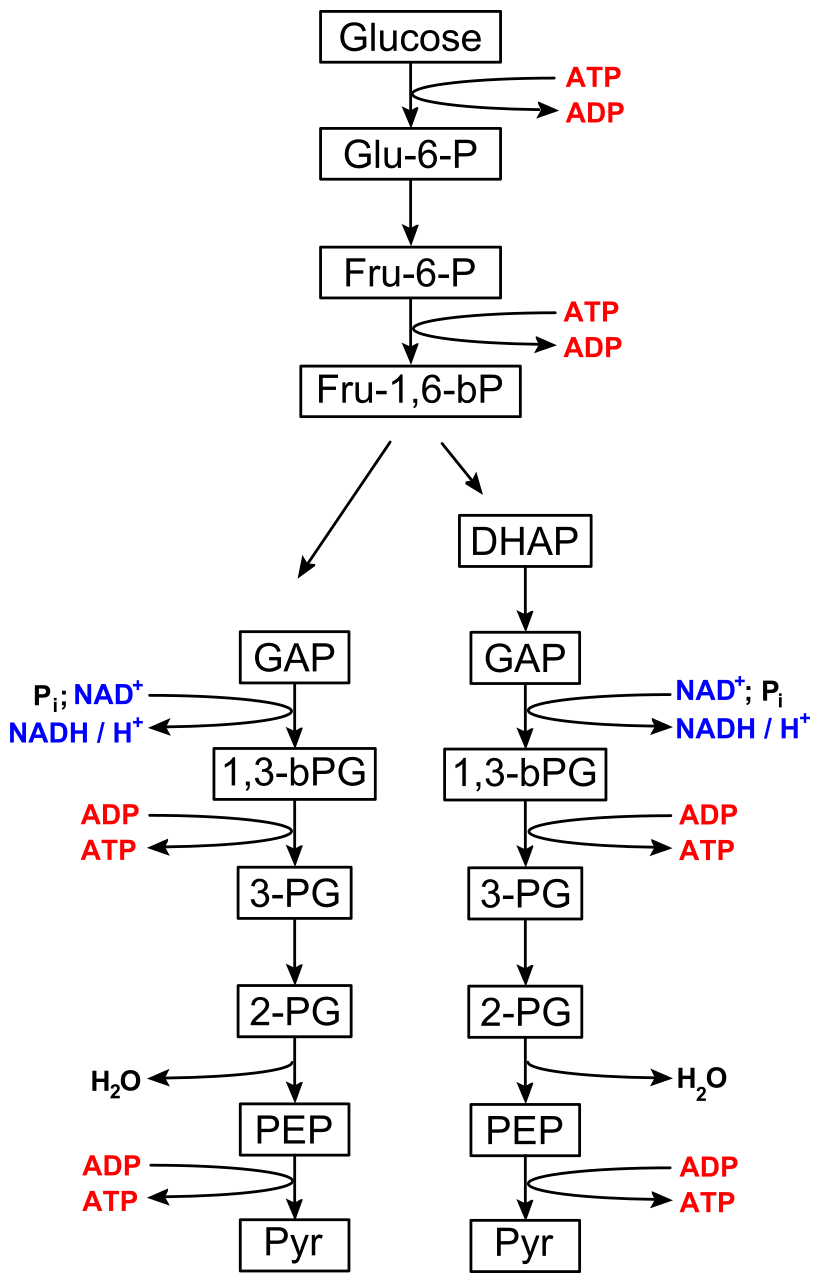
\includegraphics[height=0.75\textheight]{media/Glycolysis_overview.png}
            \caption{Glycolyse Reaktion (Wikipedia)}
        \end{figure}
    \end{minipage}%
    \begin{minipage}{0.6\textwidth}
        Reaktionsgleichungen
        \begin{itemize}[<+->]
            \item Glucose + ATP $\rightarrow$ Glu-6-P + ADP
            \item Glu-6-P $\rightarrow$ Fru-6-P
            \item Fructose-6-P + ATP $\rightarrow$ Fru-1,6-bP + ADP
            \item Fu-1,5-bP $\rightarrow$ GAP + DHAP
            \item ...
            \item Das kann schnell kompliziert werden!
        \end{itemize}
    \end{minipage}
\end{frame}


\subsection{Beispiel Einfaches System}
\begin{frame}
    \frametitle{\insertsubsection}
    \begin{minipage}{0.4\textwidth}
        \begin{figure}
            \centering
            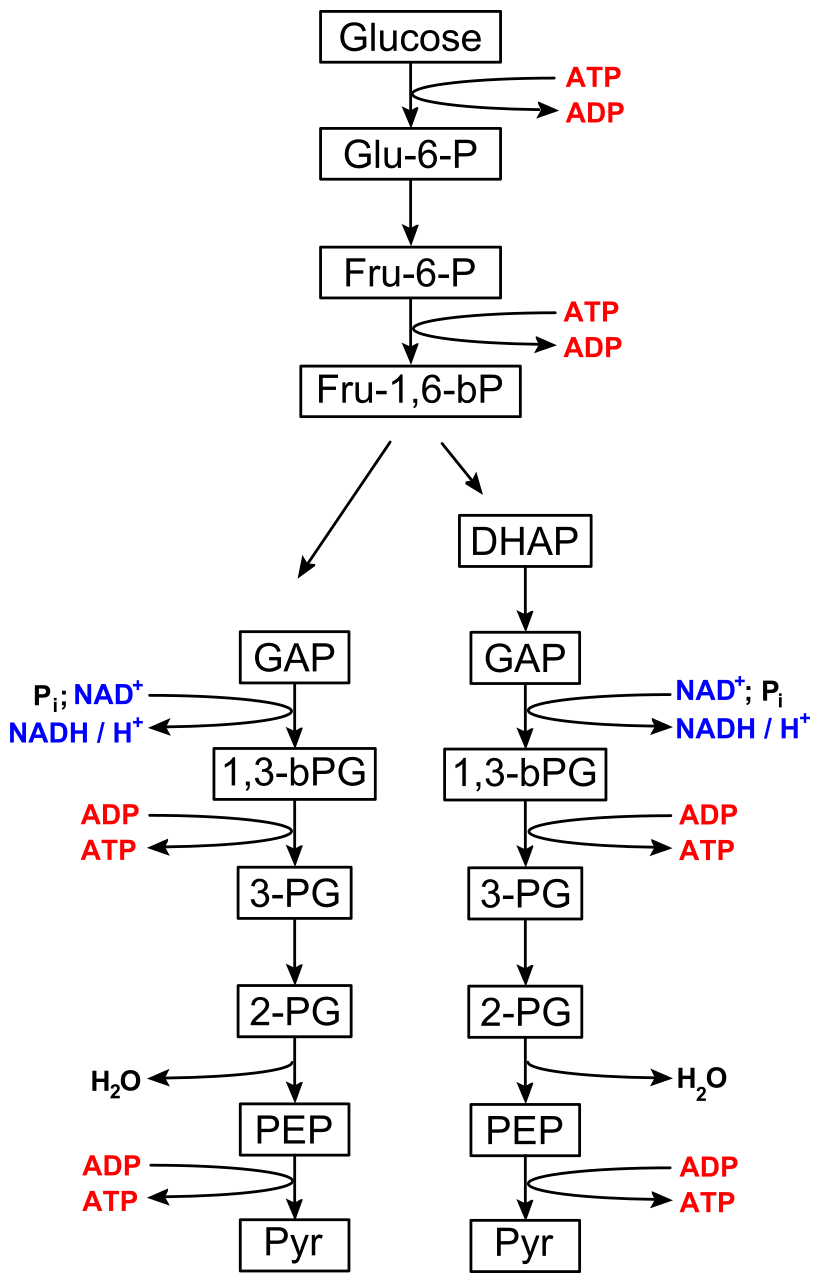
\includegraphics[height=0.75\textheight]{media/Glycolysis_overview.png}
            \caption{Glycolyse Reaktion (Wikipedia)}
        \end{figure}
    \end{minipage}%
    \begin{minipage}{0.6\textwidth}
        Reaktionsgleichungen
        \begin{itemize}[<+->]
            \item Glucose + ATP $\rightarrow$ Glu-6-P + ADP
            \item Glu-6-P $\rightarrow$ Fru-6-P
            \item Fructose-6-P + ATP $\rightarrow$ Fru-1,6-bP + ADP
            \item Fu-1,5-bP $\rightarrow$ GAP + DHAP
            \item ...
            \item Das kann schnell kompliziert werden!
        \end{itemize}
    \end{minipage}
\end{frame}


\subsection{Aufgaben an der Tafel}
\begin{frame}
    \frametitle{\insertsubsection}
    Löst die Aufgaben an der Tafel
\end{frame}